% -*- latex -*-
%%%%%%%%%%%%%%%%%%%%%%%%%%%%%%%%%%%%%%%%%%%%%%%%%%%%%%%%%%%%%%%%
%%%%%%%%%%%%%%%%%%%%%%%%%%%%%%%%%%%%%%%%%%%%%%%%%%%%%%%%%%%%%%%%
%%%%
%%%% This text file is part of the theory writeup on the
%%%% Integrative Model for Parallelism,
%%%% copyright Victor Eijkhout (eijkhout@tacc.utexas.edu) 2014-6
%%%%
%%%% shortsoftware.tex : include file for IMP-11
%%%%
%%%%%%%%%%%%%%%%%%%%%%%%%%%%%%%%%%%%%%%%%%%%%%%%%%%%%%%%%%%%%%%%
%%%%%%%%%%%%%%%%%%%%%%%%%%%%%%%%%%%%%%%%%%%%%%%%%%%%%%%%%%%%%%%%
In this section we present the outline of a software implementation
of the above theoretical notions. At first we consider the
motivating example, then we discuss in more detail the
implementation of the $I_f$ function.

\Level 2 {Basic constructs}

There are many ways of creating a distribution. The simplest
is a block distribution with even distribution of points:
\begin{verbatim}
IMP_distribution *blocked = 
      new IMP_block_distribution(decomp,globalsize);
\end{verbatim}
(We do not go into the \n{decomp} object, which keeps track of
processors, threads, and any topology on those.)

Given a distribution, creating an object is simple:
\begin{verbatim}
IMP_object *input_vector = new IMP_object( blocked );
IMP_object *output_vector = new IMP_object( blocked );
\end{verbatim}

Defining a kernel takes a couple of steps. The basic
definition takes two vectors; after that we specify the function
that is executed locally after the $\alpha\rightarrow\beta$ communication:
\begin{verbatim}
IMP_kernel *update_step = 
  new IMP_kernel(input_vector,output_vector);
update_step->localexecutefn = &threepoint_execute;
\end{verbatim}

The trickiest part is specifying the mechanism by which the $\beta$-distribution
is constructed. For a threepoint kernel that is by three shift operators:
\begin{verbatim}
update_step->add_beta_oper( new ioperator(">>1") );
update_step->add_beta_oper( new ioperator("<<1") );
update_step->add_beta_oper( new ioperator("none") );
\end{verbatim}

For a general sparse matrix we let the beta distribution be derived
from the adjacency matrix:
\verbatimsnippet{spmvpkernel}

\Level 2 {Execution}

The general execution mechanism collects the kernels into an algorithm:
\begin{verbatim}
IMP_algorithm* algorithm = 
      new IMP_algorithm(decomp);
algorithm->add_kernel( step,update_step );
\end{verbatim}
on which we perform analysis, and which,
by the inspector-executor model, can be executed multiple times:
\begin{verbatim}
algorithm->analyze_dependencies();
algorithm->execute();
\end{verbatim}

\Level 2 {Local code: global programming}

So far we have not addressed the local function that is evaluated in a
kernel. In keeping with the mode-independent nature of our model, this
function is also specified without reference to the nature of
parallelism.

To explain why the type of parallelism figures in this question, consider
the threepoint kernel
\[ y_i = x_{i-1}+x_i+x_{i+1} \]
which would be coded sequentially as
\begin{verbatim}
for (i=0; i<N; i++)
  y[i] = x[i-1] + x[i] + x[i+1]
\end{verbatim}
with some exception for the edge cases.

Using OpenMP tasks this would become:
\begin{verbatim}
ilo = lower_bound(p); ihi = upper_bound(p);
for (i=ilo; i<ihi; i++)
  y[i] = x[i-1] + x[i] + x[i+1]
\end{verbatim}
where $p$ is the abstract `process number' as used in
section~\ref{imp11example}.

In MPI the local indices would be start numbering at zero, giving code
\begin{verbatim}
myN = local_size(p);
for (i=0; i<myN; i++)
  y[i] = x[i-1] + x[i] + x[i+1]
\end{verbatim}
except that on all but the first processor we have a halo region which
is itself zero-based\footnote{One of the very few cases where Fortran
  offers an easy way out!}:
\begin{verbatim}
myN = local_size(p);
for (i=0; i<myN; i++)
  y[i] = x[i] + x[i+1] + x[i+2]
\end{verbatim}

The whole of this mess goes away in \ac{IMP}: the code for a damped
central difference is for instance:
%
\verbatimsnippet{centraldiff}
%
where the offsets and bounds are boilerplate code that is independent
of the parallelism mode.

\Level 0 {Test application: Conjugate gradient}

We have implemented a conjugate gradient algorithm. The following snippet shows how
algorithm steps are added to the algorithm. Kernels such as innerproducts and vector updates
are given here as user-level primitives; however, they are easily implemented in the \ac{IMP}
basic system as shown in examples in section~\ref{imp11apps}.
%
\verbatimsnippet{cgtemplate}

The algorithm is analyzed and executed:
\begin{verbatim}
algorithm->analyze_dependencies();
algorithm->optimize();
algorithm->execute();
\end{verbatim}

A preliminary test shows scaling comparable to PETSc:

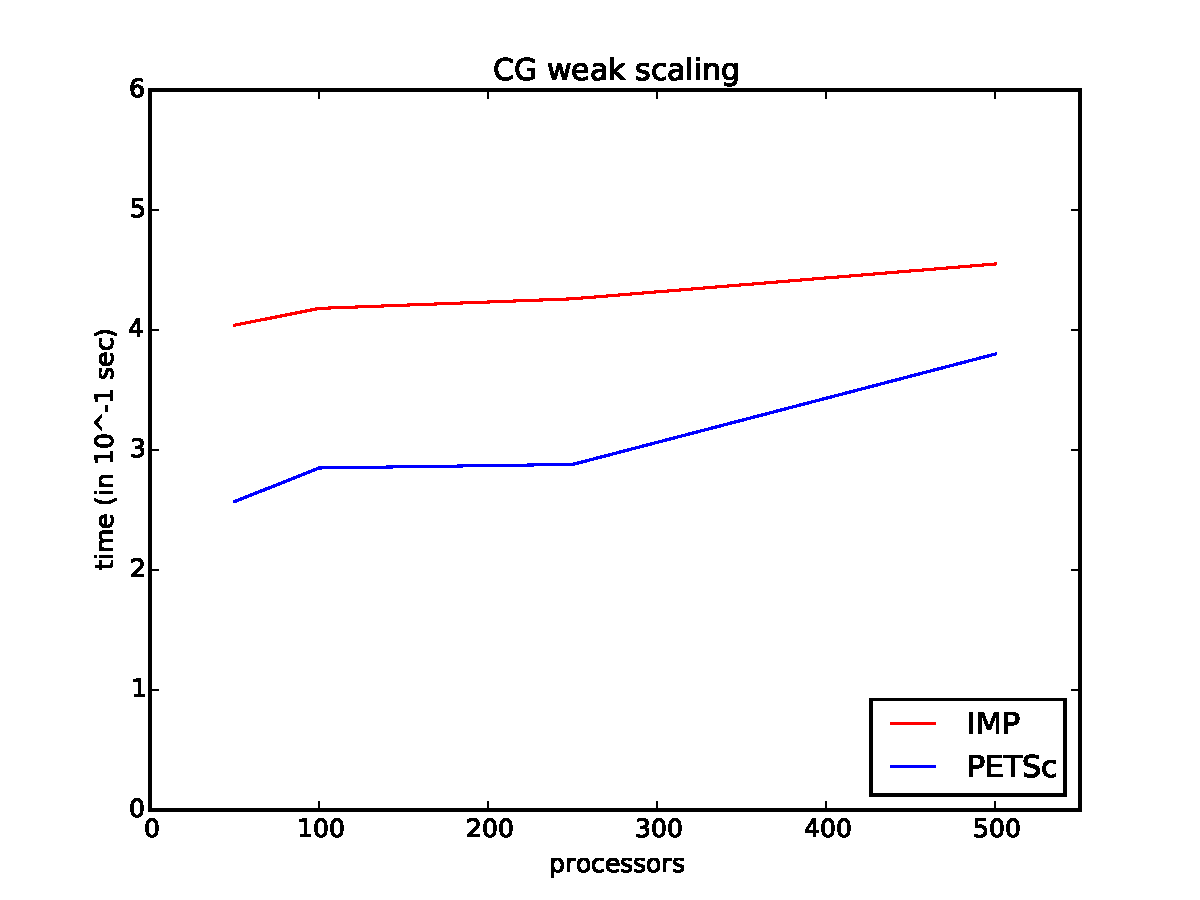
\includegraphics[scale=.5]{cg_mpi_scaling}

The performance is lower than PETSc, but this is due to the fact that
the \ac{IMP} code has very little hardwired and almost everything
derived from the algorithm. This leaves plenty of space for optimizations.

We briefly remark on collectives. Semantically, IMP will interpret a collective such
as an all-reduce as the sum of its dependencies, and therefore implement it as
as series of sends and receives. This is very inefficient, so we added a grouping
mechanism to \ac{IMP}: 
\begin{itemize}
\item an all-reduce starts as all-to-all sends and receives in process groups,
\item followed by all-to-all reducing the groups.
\end{itemize}
Effectively, this reduces the $O(P^2)$ messages of the strict implementation
to $O(P\sqrt P)$, where optimally it would be $O(P\log_2 P)$.
\begin{itemize}
\item Part of our performance loss is due to this log-versus-root order of complexity;
\item with some more sophistication we can achieve the logarithm;
\item our approach has the advantage that all operations in the reduction
  are actually tasks in the \ac{IMP} model.
\end{itemize}
